\subsection{Toolset/Innovationsplattformen/Werkzeuge} \label{toolset}

In den letzten 45 Jahren haben sich die SAP-Technologien durch kontinuierliche Veränderungen an die Anforderungen der digitalen Welt angepasst. Die Anfänge der Datenverarbeitung von SAP basierte in den 1960er Jahren auf lokalen PCs und der Mainframe-Architektur. Mit der Client-Server-Architektur und dem darauf basierenden R/3-System konnte die Software ab den 1990er Jahren eine größere Vernetzung und somit einen größeren Informationsaustausch ermöglichen. Mit der Verbreitung des Internets und dem Ausbau des mobilen Breitbandnetzes begann zwischen 2000 und 2010 mit den Technologien wie Cloud, Mobile und Big Data eine digitale Transformation \citep[S. 44]{Elsner2018}. Mit der rasant wachsenden Datenmenge entstanden Möglichkeiten, diese intelligent zu vernetzen und einen Mehrwert daraus zu schöpfen.
SAP Scloud Platform bildet die technologische Basis für die digitale Transformation mit SAP.
HANA-Anwendungen auf Microservice-Ebene für die Verarbeitung von Massendaten

Die bereits mehrfach erwähnten Cloud-Dienste: Erwähnenen, dass IaaS, PaaS notwendig ist und evtl auch SaaS in SCP
Im folgenden Kapitel werden ausgewählte Plattformen und deren Eigenschaften beschrieben.

\subsubsection{SAP Cloud Platform} \label{scp}

Die \acf{scp} ist eine offene \ac{paas}, die eine Entwicklungs- und Laufzeitumgebung für cloud-native Anwendungen bereitstellt und das Rückgrat der Services des SAP Leonardo Portfolios bildet. Unterstützt wird der Betrieb von verschiedenen Global Playern unter den Infrastrukturanbietern wie \ac{aws}, \ac{gcp}, SAP oder Microsoft Azure. Die Anwendungen können mittels verfügbarer Microservices einfach in das SAP-Backend aber auch in heterogene Systemquellen integriert werden. Somit können die Anwendungen zum Beispiel Erweiterungen für die On-Premise-Systeme sowie für \ac{saas} darstellen \citep{Acharya2019}.
Die verfügbaren Dienste der \ac{scp} können in drei Cloud-Service-Modelle unterteilt werden:

\paragraph{SAP HANA AppServices}
\paragraph{SAP HANA DB Services}
 welche Datenbank- und Applikationsdienste für bereitstellt.
Die SAP Cloud Platform ist eine offene PaaS, die auch SaaS für Kunden bereitstellt.

\begin{itemize}
  \item Cloud-Service-Modelle Utecht2018
  \item SAP HANA AppServices für Erweiterung von Cloud und Onpremise Anwendungen -> bauen auf Möglichkeiten von SAP HANA DB Services auf
  \item SAP HANA DB Services Bereitstellung von SAP HANA und Hardwar
  \item SAP HANA Infrastructure Services schneller Einsatz von SAP HANA Instanzen mit SAP Cloud Platform Integration für Backend Integration
  \item IaaS lohnt für SAP nicht da Amazon, Google und Microsoft untereinander aufgeteilt
  \item PaaS: Global Player wie IBM, HP, SAP, Pivotal haben sich für eine Basis entschieden: Cloud Foundry
  \item CF: Open Source Multi Cloud Application Platform as a Service von der CF Foundation verwaltet
  \item Entwickelt von VMWare und General Electric
  \item Gemeinsame Basis: Interoperabilitätund weniger risikoo für Abhänfifkeiten vom Anbieter
  \item SCP: einzige Platform aufbauend auf InMemory Technologie Stand 2018
  \item Business Services: als MS/API -> zentraler Ort SAP API Business Hub
  \item Verschmelzung von IaaS und PaaS -> Einfacher, Services von Überall her zu nutzen
\end{itemize}




SAP Cloud Platform und AWS Microservices und APIs
Programmiersprachen und Laufzeitumgebungen
alle gängigen IaaS können zum deployen genutzt werden
Entwicklungsumgebung SAP Web IDE und Laufzeitumgebungen
CF, NEO, ABAP
Destinationsss
Innovationsplattform
Functional Services und Business Services
Cloud-to-Cloud Integration möglich (Elsner S.247) um Kompetenzen zu vereinen. z.B. Telekom Cloud mit SCP
Embedded Platform as a Service mit zwei Lösungsvarianten. SAP Cloud Platform - Neo Environment and SAP Cloud Platform - Cloud Foundry Environment
Datenbankservices wie verschiedene SAP-HANA-Versionen, MongoDB, PostgreSQL usw
Portalservices: Fiori Launchpad als Anwendungsportal
Application Runtime als Java-Anwendung oder XS-Anwendung Entwicklung mit WEB IDE
Konnektivitätsservice: SAP Cloud Platform Integration
\ac{api}

\begin{quotation}
  cf push - and your app is alive -> in die Systemanalyse
\end{quotation}
\subsubsection{SAP Leonardo}

Die SAP Cloud Platform bildet die technologische Grundlage für die digitale Transformation mit SAP. Diese Technologien werden um die \textit{SAP-Leonardo-Technologien} ergänzt. Der Begriff lehnt sich an den Innovationsgeist Leonardo da Vincis an und soll die \textit{digitale Rennaissance} mit SAP  darstellen \citep{Howells2017}. Es gilt zu betonen, dass SAP Leonardo nicht als Plattform oder Produkt zu verstehen ist. Es handelt sich vielmehr um eine Sammlung von Functional Services (Vgl.\ref{cloud} Microservices) und Anwendungen der \ac{scp}, die als zukunftsgestaltende Technologien gelten \citep{Elsner2018}. Zu diesen Technologien gehören neben dem Internet der Dinge (\acf{iot}) auch Machine Learning, Big Data, Blockchain und Advanced Analytics. Wie bereits zuvor erwähnt, sind diese Technologien in ihrem Wesen nicht neu. Der innovative Charakter entsteht erst durch die Fähigkeit, die zusammenhängenden Technologien miteinander zu verknüpfen \citep{Utecht2018}. Für den Zweck bietet SAP vierlei Lösungen:
\begin{figure}[ht]
  \centering
  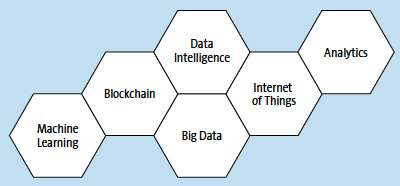
\includegraphics[width=1.0\linewidth]{sap_leonardo.png}
  \caption{Das Zusammenspiel der SAP-Leonardo-Technologien \citep[S. 87]{Elsner2018}}
\end{figure}
 \\Einerseits haben Kunden die Möglichkeit, fertige Lösungen \textit{Powered by SAP Leonardo} zu erwerben, welche nur noch an die Anforderungen des Unternehmens angepasst werden müssen \citep{Utecht2018}. Beispiele für solche Anwendungen sind \textit{Connected Goods}, \textit{Connected Assets} oder \textit{Connected Infrastructure} \citep{Elsner2018}. Mit der Cloud-Anwendung \textit{SAP Leonardo Bridge} können die Daten aus diesen \ac{iot}-Anwendungen mit den Backend-Daten zugesammengeführt, dargestellt und verarbeitet werden. Das Produkt \ac{iot}-Edge ist die Schnittstelle zwischen den Sensoren am Gerät und der Cloud. Bevor die Daten an die Cloud übertragen werden, können sie im Offline-Betrieb gepuffert, aggregiert und vorverarbeitet werden \citep{Utecht2018}.
\\Allerdings können \ac{iot}-Szenarien mit der \textit{SAP Leonardo IoT Foundation} agil selbst entwickelt werden \citep{Elsner2018}. Hierfür ist eine Sammlung von Microservices und \ac{api}s auf der \ac{scp} bereitgestellt. Diese können für das \textit{Thing Management} und \textit{SAP IoT Application Enablement} verwendet werden. Im \textit{Thing Management} werden die Geräte nach einem vorgedachten Modell verwaltet, für die im \textit{Application Enablement} ein \textit{digitaler Zwilling} als Grundlage für die Anwendungsentwicklung erstellt wird \citep{Elsner2018}.
\\Im Grunde ist SAP Leonardo ein Sammelbegriff für alle \ac{iot}-relevanten Produkte \citep{Utecht2018}. Kennzeichnend für die Innovation ist neben der Interoperabilität der Services die Interoperabilität der Unternehmensdaten. Das Unternehmensgedächtnis ist in dem digitalen Kern, also dem \ac{erp}-System, verankert \citep{Elsner2018}. Der digitale Kern kann nahtlos mit der agilen Entwicklung auf dem \textit{Digital Innovation System} verbunden werden. Mithilfe  z.B von SAP zur Verfügung gestellten Design Thinking Methoden können aus kontextbezogenen Stamm- und Historiendaten des Unternehmens Erkenntnisse für Geschäftsprozesse geschlossen werden \citep{Elsner2018}.
\\SAP spricht von einem Ökosystem, in dem Entwicklungs- und Implementierungspartner mit den Technologien interagieren, um innovative und effiziente Produkte zu erzeugen. Während Implementierungspartner dabei helfen, bereits bestehende Lösungen und Anwendungen zu konfigurieren und anzupassen, entwickeln die Entwicklungspartner auf Basis der SAP-Leonardo-Technologien neue Anwendungen. Dies ist vor allem im Kontext der Verschmelzung der IT mit dem Maschinenbau und der Elektrotechnik interessant. Die Konvergenz der Themenfelder bewegt reine Hardwarehersteller zu der Entwicklung von intelligenten Softwarelösungen als digitale Service Provider \citep{Elsner2018}. Das Ökosystem beinhaltet zudem die in Abschnitt \ref{scp} erwähnten Infrastrukturpartner, Softwaredienste und Laufzeitumgebungen aber auch z.B. Standards und Normen.


\subsubsection{AWS Cloud}
Größte Public Cloud der Welt
SNS-Server
Außerdem basiert SCP auf AWS

\subsubsection{Git}

\newpage
